\documentclass[10.5pt,a4paper]{article}

\usepackage[utf8]{vietnam}
\usepackage{mathptmx}
\usepackage{geometry}
\geometry{
    a4paper,
    top=18mm,
    bottom=18mm,
    left=20mm,
    right=18mm,
    headheight=14pt
}

\usepackage{amsmath,amssymb,amsfonts}
\usepackage{graphicx}
\graphicspath{{../figures/}{../../figures/}{./figures/}{figures/}}
\usepackage{booktabs}
\usepackage{tabularx}
\usepackage{array}
\usepackage{float}
\usepackage{setspace}
\setstretch{1.12}

\usepackage{fancyhdr}
\pagestyle{fancy}
\fancyhf{}
\fancyhead[L]{\slshape \small Đồ án 1: Trào lưu công suất Newton--Raphson (EE3810E)}
\fancyhead[R]{\slshape \small Bài tập tự tính tay \& Checkpoint đối chiếu}
\fancyfoot[C]{\small Trang \thepage / 4}
\renewcommand{\headrulewidth}{0.4pt}
\renewcommand{\footrulewidth}{0pt}

\usepackage{xcolor}
\definecolor{hustblue}{RGB}{0, 32, 96}
\definecolor{hustred}{RGB}{180, 0, 0}
\definecolor{darkgreen}{RGB}{0, 100, 40}
\definecolor{graybg}{RGB}{245, 247, 250}

\usepackage{hyperref}
\hypersetup{
    colorlinks=true,
    linkcolor=hustblue,
    citecolor=hustblue,
    urlcolor=blue
}

\begin{document}

% ==================== TRANG 1: THÔNG SỐ ĐỀ BÀI ====================
\begin{center}
    {\fontsize{10}{12}\selectfont \textbf{ĐẠI HỌC BÁCH KHOA HÀ NỘI --- TRƯỜNG ĐIỆN - ĐIỆN TỬ --- BỘ MÔN HỆ THỐNG ĐIỆN}}\\[2pt]
    {\fontsize{9}{11}\selectfont HỌC PHẦN: ĐỒ ÁN 1 (EE3810E) --- NĂM HỌC 2026}\\[6pt]
    \hrule height 1.2pt
    \vspace{6pt}
    {\fontsize{13}{16}\selectfont \textcolor{hustblue}{\textbf{PHIẾU BÀI TẬP TỰ HỌC \& TÍNH TOÁN THỦ CÔNG TỪNG BƯỚC}}}\\[3pt]
    {\fontsize{11}{14}\selectfont \textbf{BÀI TOÁN TRÀO LƯU CÔNG SUẤT XÁC LẬP BẰNG PHƯƠNG PHÁP NEWTON--RAPHSON}}\\[2pt]
    {\fontsize{9.5}{12}\selectfont \textit{(Mô hình tọa độ cực --- Lưới truyền tải chuẩn 3 nút --- Kiểm chứng Bước lặp 1)}}\\[6pt]
    \hrule height 0.6pt
\end{center}

\vspace{-4pt}
\subsection*{I. MỤC TIÊU VÀ HƯỚNG DẪN TỰ HỌC}
\vspace{-4pt}
Tài liệu được thiết kế theo phương pháp luận "hộp trắng" (white-box) giúp sinh viên tự rèn luyện kỹ năng tính toán, nắm vững bản chất toán học của phương pháp Newton--Raphson và tự tin làm chủ các bộ phần mềm giải số:
\begin{itemize}\setlength{\itemsep}{1pt}\setlength{\parskip}{0pt}
    \item \textbf{Chuẩn bị:} Máy tính bỏ túi (Casio fx-580VNX / fx-880BTG), giấy nháp và bút.
    \item \textbf{Phương pháp:} Đọc thông số và công thức $\to$ Tự tính toán các câu hỏi ở Mục IV ra giấy nháp $\to$ Tra cứu đối chiếu với Bảng Checkpoints ở Trang 4 để tự chấm điểm độ chính xác.
\end{itemize}

\vspace{-4pt}
\subsection*{II. THÔNG SỐ LƯỚI ĐIỆN TRUYỀN TẢI CHUẨN 3 NÚT}
\vspace{-4pt}
Lưới điện 3 nút có công suất cơ bản $S_{\text{base}} = 100.0\text{ MVA}$, gồm 3 thanh cái và 3 đường dây (Hình~\ref{fig:3bus_sld}).

\begin{figure}[H]
\centering
\vspace{-6pt}
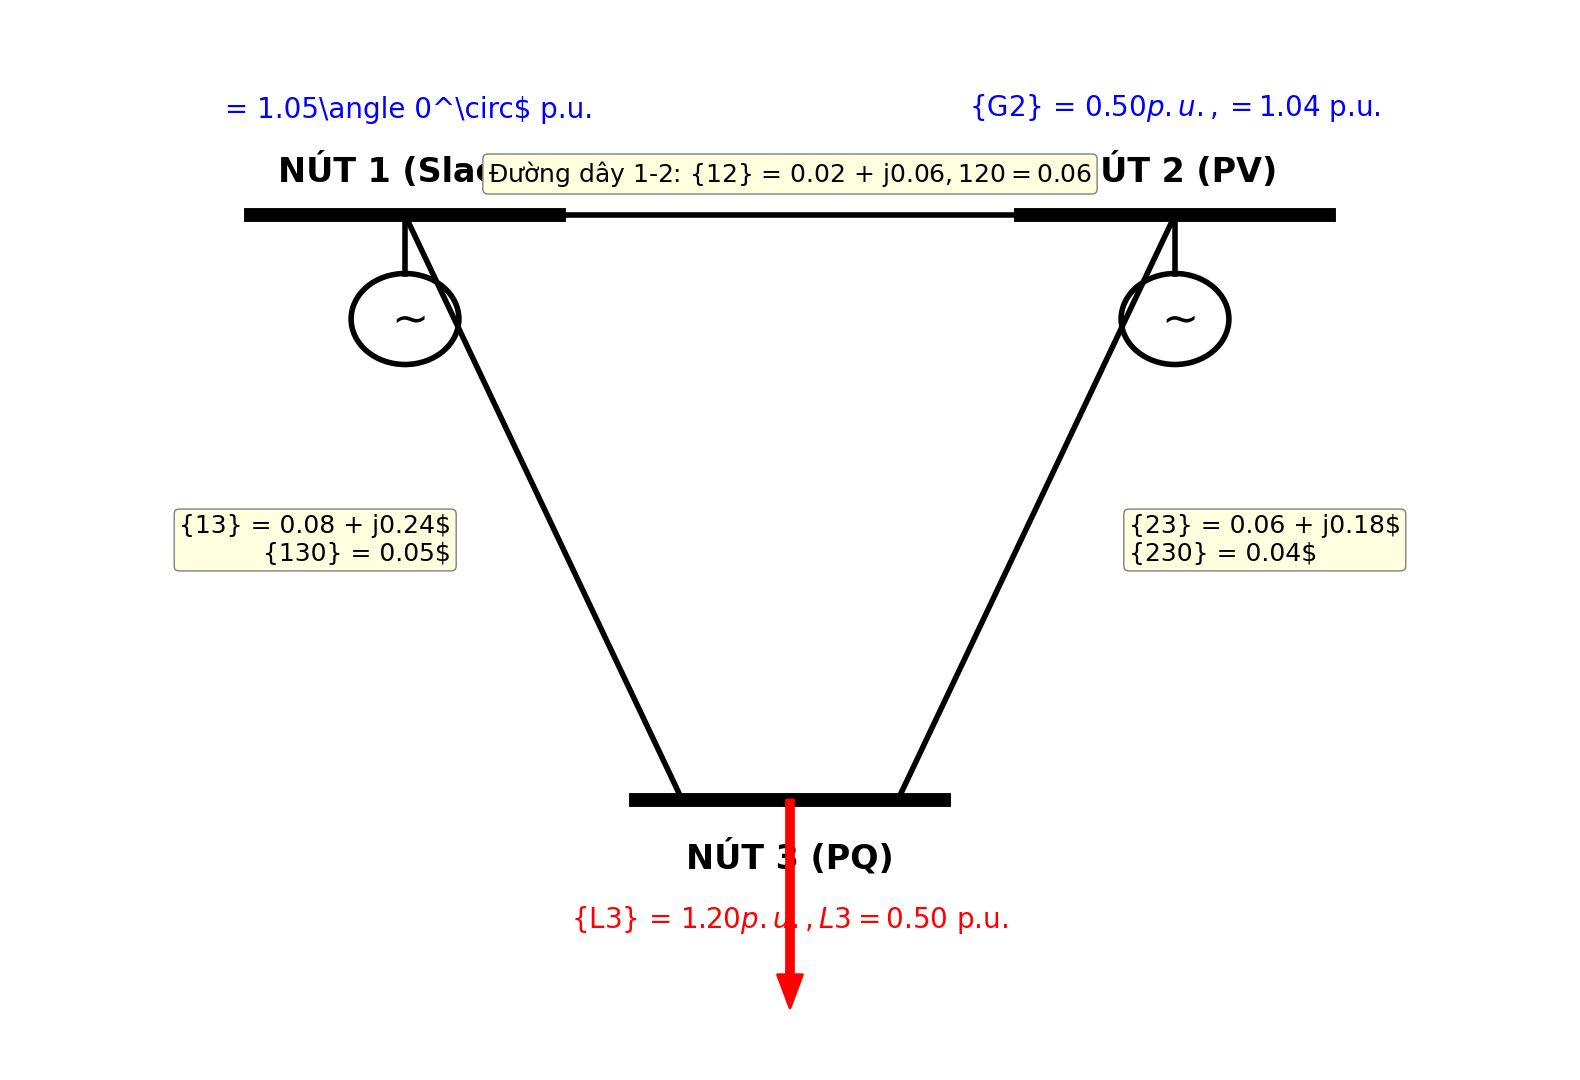
\includegraphics[width=0.52\textwidth]{3bus_network_vi.png}
\vspace{-8pt}
\caption{Sơ đồ một sợi hệ thống điện truyền tải mẫu 3 nút.}
\label{fig:3bus_sld}
\end{figure}

\vspace{-12pt}
\subsubsection*{1. Bảng thông số nút (Bus Data)}
\vspace{-4pt}
\begin{table}[H]
\centering
\small
\begin{tabular}{ccccccc}
\toprule
\textbf{Nút} & \textbf{Loại nút} & $U_i\text{ (p.u.)}$ & $\delta_i\text{ (rad)}$ & $P_{Gi}\text{ (p.u.)}$ & $P_{Li}\text{ (p.u.)}$ & $Q_{Li}\text{ (p.u.)}$ \\
\midrule
\textbf{1} & Slack (Cân bằng) & $1.05$ & $0.0000$ & Cần tìm & $0.00$ & $0.00$ \\
\textbf{2} & PV (Máy phát) & $1.04$ & Cần tìm & $0.50$ ($50\text{ MW}$) & $0.00$ & $0.00$ \\
\textbf{3} & PQ (Phụ tải) & Cần tìm & Cần tìm & $0.00$ & $1.20$ ($120\text{ MW}$) & $0.50$ ($50\text{ Mvar}$) \\
\bottomrule
\end{tabular}
\end{table}

\vspace{-6pt}
\noindent $\blacktriangleright$ \textbf{Công suất ấn định đặt vào các nút ($P_i^{\text{spec}} = P_{Gi} - P_{Li}$, $Q_i^{\text{spec}} = Q_{Gi} - Q_{Li}$):}
$$P_2^{\text{spec}} = 0.50 - 0.00 = \mathbf{0.50\text{ p.u.}}, \quad P_3^{\text{spec}} = 0.00 - 1.20 = \mathbf{-1.20\text{ p.u.}}, \quad Q_3^{\text{spec}} = 0.00 - 0.50 = \mathbf{-0.50\text{ p.u.}}$$

\vspace{-6pt}
\subsubsection*{2. Bảng thông số nhánh đường dây (Branch Data)}
\vspace{-4pt}
Đường dây mô hình $\pi$ tương đương, $B_{ij0}$ là tổng dung dẫn nạp nối đất ($b_{ij0}/2 = B_{ij0}/2$ tại mỗi đầu thanh cái):
\begin{table}[H]
\centering
\small
\begin{tabular}{ccccc}
\toprule
\textbf{Nhánh} & \textbf{Từ nút -- Đến nút} & Điện trở $R_{ij}\text{ (p.u.)}$ & Điện kháng $X_{ij}\text{ (p.u.)}$ & Dung dẫn nạp $B_{ij0}\text{ (p.u.)}$ \\
\midrule
1 & $1 - 2$ & $0.02$ & $0.06$ & $0.06$ \\
2 & $1 - 3$ & $0.08$ & $0.24$ & $0.05$ \\
3 & $2 - 3$ & $0.06$ & $0.18$ & $0.04$ \\
\bottomrule
\end{tabular}
\end{table}

\clearpage

% ==================== TRANG 2: CÔNG THỨC & HƯỚNG DẪN MÁY TÍNH ====================
\subsection*{III. TÓM TẮT CƠ SỞ TOÁN HỌC \& CÔNG THỨC TRỌNG TÂM}
\vspace{-4pt}

\subsubsection*{1. Ma trận dẫn nạp nút $\mathbf{Y}_{\text{bus}}$}
\vspace{-4pt}
\begin{itemize}\setlength{\itemsep}{1pt}\setlength{\parskip}{0pt}
    \item Dẫn nạp nối tiếp: $y_{ij} = \dfrac{1}{R_{ij} + jX_{ij}} = g_{ij} + jb_{ij} = \dfrac{R_{ij}}{R_{ij}^2 + X_{ij}^2} - j \dfrac{X_{ij}}{R_{ij}^2 + X_{ij}^2}$
    \item Ngoài đường chéo: $Y_{ij} = -\, y_{ij} = G_{ij} + jB_{ij} \quad (i \ne j)$. Do mạng điện song phương nên $Y_{ij} = Y_{ji}$.
    \item Trên đường chéo: $Y_{ii} = \sum_{j \in \Omega_i} y_{ij} + j \sum_{j \in \Omega_i} \dfrac{B_{ij0}}{2} = G_{ii} + jB_{ii}$
\end{itemize}

\vspace{-4pt}
\subsubsection*{2. Phương trình công suất nút tọa độ cực}
\vspace{-4pt}
\begin{align}
P_i(\boldsymbol{\delta}, \mathbf{U}) &= U_i^2 G_{ii} + \sum_{j \ne i} U_i U_j \left[ G_{ij} \cos(\delta_i - \delta_j) + B_{ij} \sin(\delta_i - \delta_j) \right] \\
Q_i(\boldsymbol{\delta}, \mathbf{U}) &= -\, U_i^2 B_{ii} + \sum_{j \ne i} U_i U_j \left[ G_{ij} \sin(\delta_i - \delta_j) - B_{ij} \cos(\delta_i - \delta_j) \right]
\end{align}

\vspace{-6pt}
\subsubsection*{3. Hệ phương trình đại số tuyến tính hiệu chỉnh Newton--Raphson}
\vspace{-4pt}
\begin{equation}
\begin{bmatrix}
\Delta \mathbf{P} \\
\Delta \mathbf{Q}
\end{bmatrix}
=
\begin{bmatrix}
\mathbf{H} & \mathbf{N} \\
\mathbf{M} & \mathbf{L}
\end{bmatrix}
\begin{bmatrix}
\Delta \boldsymbol{\delta} \\
\Delta \mathbf{U} / \mathbf{U}
\end{bmatrix}
\iff \mathbf{J} \cdot \Delta \mathbf{x} = \Delta \mathbf{S}
\end{equation}

\vspace{-6pt}
\subsubsection*{4. Bảng 8 công thức vi phân giải tích của ma trận Jacobian}
\vspace{-4pt}
\begin{table}[H]
\centering
\small
\begin{tabular}{lll}
\toprule
\textbf{Khối ma trận} & \textbf{Ngoài đường chéo ($i \ne j$)} & \textbf{Trên đường chéo chính ($i = j$)} \\
\midrule
$\mathbf{H} = \dfrac{\partial \mathbf{P}}{\partial \boldsymbol{\delta}}$ & $H_{ij} = U_i U_j [G_{ij} \sin\delta_{ij} - B_{ij} \cos\delta_{ij}]$ & $H_{ii} = -\, Q_i^{\text{calc}} - U_i^2 B_{ii}$ \\[6pt]
$\mathbf{N} = U \dfrac{\partial \mathbf{P}}{\partial \mathbf{U}}$ & $N_{ij} = U_i U_j [G_{ij} \cos\delta_{ij} + B_{ij} \sin\delta_{ij}]$ & $N_{ii} = P_i^{\text{calc}} + U_i^2 G_{ii}$ \\[6pt]
$\mathbf{M} = \dfrac{\partial \mathbf{Q}}{\partial \boldsymbol{\delta}}$ & $M_{ij} = -\, N_{ij}$ & $M_{ii} = P_i^{\text{calc}} - U_i^2 G_{ii}$ \\[6pt]
$\mathbf{L} = U \dfrac{\partial \mathbf{Q}}{\partial \mathbf{U}}$ & $L_{ij} = H_{ij}$ & $L_{ii} = Q_i^{\text{calc}} - U_i^2 B_{ii}$ \\
\bottomrule
\end{tabular}
\end{table}

\noindent $\blacktriangleright$ \textbf{Quy tắc rút gọn cực nhanh tại bước khởi tạo phẳng ($m=0$):}\\
Do $\delta_i = \delta_j = 0 \implies \delta_{ij} = 0 \implies \cos(0) = 1, \sin(0) = 0$, ta có:
$$H_{ij}^{(0)} = L_{ij}^{(0)} = -\, U_i U_j B_{ij}, \qquad N_{ij}^{(0)} = -\, M_{ij}^{(0)} = U_i U_j G_{ij}$$

\vspace{-4pt}
\subsection*{IV. HƯỚNG DẪN THỦ THUẬT BẤM MÁY TÍNH CASIO fx-580VNX}
\vspace{-4pt}
\begin{enumerate}\setlength{\itemsep}{2pt}\setlength{\parskip}{0pt}
    \item \textbf{Tính dẫn nạp nhánh $y_{ij}$ trong 5 giây:}
    \begin{itemize}\setlength{\itemsep}{0pt}
        \item Bấm \texttt{MENU} $\to$ \texttt{2} (Chế độ số phức \texttt{Complex}).
        \item Nhập phân số: $\dfrac{1}{0.02 + 0.06 i}$ rồi bấm phím \texttt{=}. Máy tính hiển thị ngay $5 - 15i$.
    \end{itemize}
    \item \textbf{Giải hệ phương trình tìm $\Delta \mathbf{x}$ không cần nghịch đảo ma trận:}
    \begin{itemize}\setlength{\itemsep}{0pt}
        \item Bấm \texttt{MENU} $\to$ \texttt{9} (Equation / Func) $\to$ \texttt{1} (Simul Equation) $\to$ chọn \texttt{3} (Hệ 3 ẩn số: $x, y, z$).
        \item Nhập lần lượt các hệ số hàng của $\mathbf{J}^{(0)}$ và véc-tơ cột sai lệch công suất:
        $$\begin{aligned}
        \text{Hàng 1: } & 21.58 \quad & -5.20 \quad & -1.733333 \quad & 0.482667 \\
        \text{Hàng 2: } & -5.20 \quad & 9.1375 \quad & 2.7875 \quad & -1.070833 \\
        \text{Hàng 3: } & 1.733333 \quad & -3.045833 \quad & 8.2725 \quad & -0.0675
        \end{aligned}$$
        \item Bấm \texttt{=}, máy hiển thị trực tiếp nghiệm: $x = \Delta \delta_2^{(0)}$, $y = \Delta \delta_3^{(0)}$, $z = \Delta U_3^{(0)} / U_3^{(0)}$!
    \end{itemize}
\end{enumerate}

\clearpage

% ==================== TRANG 3: CÁC CÂU HỎI THỰC HÀNH ====================
\subsection*{V. CÁC CÂU HỎI TỰ THỰC HÀNH TÍNH TAY (BƯỚC LẶP 1: $m = 0 \to 1$)}
\vspace{-4pt}

\subsubsection*{Câu 1: Xây dựng ma trận dẫn nạp nút $\mathbf{Y}_{\text{bus}}$}
\begin{enumerate}\setlength{\itemsep}{2pt}\setlength{\parskip}{0pt}
    \item[1.1] Tính giá trị bằng số phức $g_{ij} + j b_{ij}$ của 3 dẫn nạp nối tiếp: $y_{12}, y_{13}, y_{23}$.
    \item[1.2] Tính 3 phần tử dẫn nạp tương hỗ ngoài đường chéo chính: $Y_{12}, Y_{13}, Y_{23}$.
    \item[1.3] Tính 3 phần tử dẫn nạp riêng trên đường chéo chính:
    $$Y_{11} = y_{12} + y_{13} + j(b_{120}/2 + b_{130}/2)$$
    $$Y_{22} = y_{12} + y_{23} + j(b_{120}/2 + b_{230}/2)$$
    $$Y_{33} = y_{13} + y_{23} + j(b_{130}/2 + b_{230}/2)$$
    Viết lại toàn bộ ma trận dẫn nạp nút $\mathbf{Y}_{\text{bus}}$ kích thước $3 \times 3$.
\end{enumerate}

\subsubsection*{Câu 2: Thiết lập khởi tạo phẳng và xác định biến trạng thái}
\begin{enumerate}\setlength{\itemsep}{2pt}\setlength{\parskip}{0pt}
    \item[2.1] Dựa vào phân loại nút (Slack: Nút 1, PV: Nút 2, PQ: Nút 3), hãy liệt kê các biến trạng thái cần tìm của hệ phương trình Newton--Raphson. Kích thước ma trận Jacobian là bao nhiêu?
    \item[2.2] Thiết lập giá trị véc-tơ trạng thái ban đầu theo phương pháp khởi tạo phẳng (Flat Start) tại bước $m = 0$:
    $$\mathbf{x}^{(0)} = [\delta_2^{(0)}, \delta_3^{(0)}, U_3^{(0)}]^T$$
\end{enumerate}

\subsubsection*{Câu 3: Tính toán công suất nút và véc-tơ sai lệch công suất $\Delta \mathbf{S}^{(0)}$}
\begin{enumerate}\setlength{\itemsep}{2pt}\setlength{\parskip}{0pt}
    \item[3.1] Tại bước $m=0$ ($\delta_1 = \delta_2 = \delta_3 = 0, U_1 = 1.05, U_2 = 1.04, U_3 = 1.0$), hãy thế số tính:
    $$P_2^{(0)} = U_2^2 G_{22} + U_2 U_1 G_{21} + U_2 U_3 G_{23}$$
    $$P_3^{(0)} = U_3^2 G_{33} + U_3 U_1 G_{31} + U_3 U_2 G_{32}$$
    $$Q_3^{(0)} = -\, U_3^2 B_{33} - U_3 U_1 B_{31} - U_3 U_2 B_{32}$$
    \item[3.2] Tính công suất phản kháng phụ trợ $Q_2^{(0)}$:
    $$Q_2^{(0)} = -\, U_2^2 B_{22} - U_2 U_1 B_{21} - U_2 U_3 B_{23}$$
    \item[3.3] Xác định véc-tơ sai lệch công suất ban đầu:
    $$\Delta P_2^{(0)} = P_2^{\text{spec}} - P_2^{(0)}, \quad \Delta P_3^{(0)} = P_3^{\text{spec}} - P_3^{(0)}, \quad \Delta Q_3^{(0)} = Q_3^{\text{spec}} - Q_3^{(0)}$$
\end{enumerate}

\subsubsection*{Câu 4: Tính các phần tử của ma trận Jacobian $\mathbf{J}^{(0)}$}
Áp dụng bảng công thức vi phân rút gọn tại $m=0$, tính 9 giá trị số của ma trận Jacobian cấp $3 \times 3$:
\begin{itemize}\setlength{\itemsep}{1pt}\setlength{\parskip}{0pt}
    \item $H_{22} = -\, Q_2^{(0)} - U_2^2 B_{22}, \quad H_{23} = -\, U_2 U_3 B_{23}, \quad H_{32} = -\, U_3 U_2 B_{32}, \quad H_{33} = -\, Q_3^{(0)} - U_3^2 B_{33}$
    \item $N_{23} = U_2 U_3 G_{23}, \quad N_{33} = P_3^{(0)} + U_3^2 G_{33}$
    \item $M_{32} = -\, N_{32} = -\, U_3 U_2 G_{32}, \quad M_{33} = P_3^{(0)} - U_3^2 G_{33}$
    \item $L_{33} = Q_3^{(0)} - U_3^2 B_{33}$
\end{itemize}

\subsubsection*{Câu 5: Giải hệ phương trình tuyến tính và cập nhật trạng thái Bước 1}
\begin{enumerate}\setlength{\itemsep}{2pt}\setlength{\parskip}{0pt}
    \item[5.1] Lập hệ phương trình tuyến tính $\mathbf{J}^{(0)} \Delta \mathbf{x}^{(0)} = \Delta \mathbf{S}^{(0)}$ và bấm máy tính giải ra:
    $$\Delta \delta_2^{(0)}\text{ (rad)}, \quad \Delta \delta_3^{(0)}\text{ (rad)}, \quad \Delta U_3^{(0)}\text{ (p.u.)}$$
    \item[5.2] Cập nhật véc-tơ trạng thái mới sau Bước lặp 1 ($m = 1$):
    $$\delta_2^{(1)} = \delta_2^{(0)} + \Delta \delta_2^{(0)}, \quad \delta_3^{(1)} = \delta_3^{(0)} + \Delta \delta_3^{(0)}, \quad U_3^{(1)} = U_3^{(0)} + \Delta U_3^{(0)}$$
\end{enumerate}

\clearpage

% ==================== TRANG 4: BẢNG CHECKPOINTS ====================
\subsection*{VI. BẢNG CHECKPOINTS TRA CỨU ĐỐI CHIẾU KẾT QUẢ}
\vspace{-4pt}
\textit{\textcolor{hustred}{\textbf{Lưu ý:}} Hãy hoàn thành phần tự tính toán trước khi tra cứu để đạt hiệu quả ôn luyện cao nhất!}

\subsubsection*{1. Dẫn nạp nhánh và Ma trận $\mathbf{Y}_{\text{bus}}$}
\vspace{-4pt}
\begin{itemize}\setlength{\itemsep}{1pt}\setlength{\parskip}{0pt}
    \item $y_{12} = \mathbf{5.000000 - j 15.000000\text{ p.u.}}, \quad y_{13} = \mathbf{1.250000 - j 3.750000\text{ p.u.}}, \quad y_{23} = \mathbf{1.666667 - j 5.000000\text{ p.u.}}$
\end{itemize}
\vspace{-4pt}
\begin{equation}
\mathbf{Y}_{\text{bus}} =
\begin{bmatrix}
6.250000 - j18.695000 & -5.000000 + j15.000000 & -1.250000 + j3.750000 \\
-5.000000 + j15.000000 & 6.666667 - j19.950000 & -1.666667 + j5.000000 \\
-1.250000 + j3.750000 & -1.666667 + j5.000000 & 2.916667 - j8.705000
\end{bmatrix}
\end{equation}

\vspace{-6pt}
\subsubsection*{2. Công suất tính toán và sai lệch công suất tại bước $m=0$}
\vspace{-4pt}
\begin{itemize}\setlength{\itemsep}{1pt}\setlength{\parskip}{0pt}
    \item $P_2^{(0)} = \mathbf{0.017333\text{ p.u.}}, \quad P_3^{(0)} = \mathbf{-0.129167\text{ p.u.}}, \quad Q_3^{(0)} = \mathbf{-0.432500\text{ p.u.}}, \quad Q_2^{(0)} = \mathbf{-0.002080\text{ p.u.}}$
    \item $\Delta P_2^{(0)} = 0.500000 - 0.017333 = \mathbf{+0.482667\text{ p.u.}}$
    \item $\Delta P_3^{(0)} = -1.200000 - (-0.129167) = \mathbf{-1.070833\text{ p.u.}}$
    \item $\Delta Q_3^{(0)} = -0.500000 - (-0.432500) = \mathbf{-0.067500\text{ p.u.}}$
\end{itemize}

\vspace{-6pt}
\subsubsection*{3. Ma trận Jacobian $\mathbf{J}^{(0)}$ và nghịch đảo $[\mathbf{J}^{(0)}]^{-1}$}
\vspace{-4pt}
\begin{equation}
\mathbf{J}^{(0)} =
\begin{bmatrix}
21.580000 & -5.200000 & -1.733333 \\
-5.200000 & 9.137500 & 2.787500 \\
1.733333 & -3.045833 & 8.272500
\end{bmatrix}, \qquad
[\mathbf{J}^{(0)}]^{-1} =
\begin{bmatrix}
0.053703 & 0.030848 & 0.000858 \\
0.030562 & 0.115943 & -0.032665 \\
0.000000 & 0.036225 & 0.108676
\end{bmatrix}
\end{equation}

\vspace{-6pt}
\subsubsection*{4. Véc-tơ hiệu chỉnh và Cập nhật trạng thái sau Bước lặp 1}
\vspace{-4pt}
\begin{itemize}\setlength{\itemsep}{1pt}\setlength{\parskip}{0pt}
    \item $\Delta \delta_2^{(0)} = \mathbf{-0.007170\text{ rad}} \quad (-0.4108^\circ)$
    \item $\Delta \delta_3^{(0)} = \mathbf{-0.107200\text{ rad}} \quad (-6.1421^\circ)$
    \item $\Delta U_3^{(0)} = \mathbf{-0.046127\text{ p.u.}}$
\end{itemize}
$\blacktriangleright$ \textbf{Véc-tơ trạng thái sau Bước lặp 1 ($m=1$):}
$$\delta_2^{(1)} = \mathbf{-0.007170\text{ rad}} \quad (-0.4108^\circ), \qquad \delta_3^{(1)} = \mathbf{-0.107200\text{ rad}} \quad (-6.1421^\circ), \qquad U_3^{(1)} = \mathbf{0.953873\text{ p.u.}}$$

\vspace{-6pt}
\subsubsection*{5. Bảng trạng thái xác lập sau khi hội tụ (4 bước lặp, chuẩn sai số $\Vert \mathbf{f} \Vert_\infty \le 10^{-10}\text{ p.u.}$)}
\vspace{-4pt}
\begin{table}[H]
\centering
\small
\begin{tabular}{ccccccc}
\toprule
\textbf{Nút} & $U_i\text{ (p.u.)}$ & $\delta_i\text{ (rad)}$ & $\delta_i\text{ (độ)}$ & $P_i\text{ (MW)}$ & $Q_i\text{ (Mvar)}$ & \textbf{Vai trò} \\
\midrule
\textbf{1} & $1.050000$ & $0.000000$ & $0.0000^\circ$ & $+76.4522$ & $+34.9226$ & Nút cân bằng (Slack) \\
\textbf{2} & $1.040000$ & $-0.008612$ & $-0.4934^\circ$ & $+50.0000$ & $+18.9489$ & Nút máy phát (PV) \\
\textbf{3} & $0.944383$ & $-0.114287$ & $-6.5482^\circ$ & $-120.0000$ & $-50.0000$ & Nút phụ tải (PQ) \\
\bottomrule
\end{tabular}
\end{table}

\vspace{-6pt}
\subsubsection*{6. Phân bố công suất nhánh và Tổn thất truyền tải sau hội tụ}
\vspace{-4pt}
\begin{table}[H]
\centering
\small
\begin{tabular}{crrrrrr}
\toprule
\textbf{Đường dây} & $P_{ij}\text{ (MW)}$ & $Q_{ij}\text{ (Mvar)}$ & $P_{ji}\text{ (MW)}$ & $Q_{ji}\text{ (Mvar)}$ & $\Delta P_{ij}\text{ (MW)}$ & $\Delta Q_{ij}\text{ (Mvar)}$ \\
\midrule
$1 - 2$ & $19.3765$ & $7.8011$ & $-19.2860$ & $-14.0820$ & $0.0905$ & $-6.2808$ \\
$1 - 3$ & $57.0761$ & $27.1212$ & $-54.0645$ & $-23.0723$ & $3.0116$ & $4.0489$ \\
$2 - 3$ & $69.2850$ & $33.0310$ & $-65.9350$ & $-26.9277$ & $3.3501$ & $6.1033$ \\
\midrule
\textbf{Tổng tổn thất} & -- & -- & -- & -- & $\mathbf{6.4522\text{ MW}}$ & $\mathbf{3.8715\text{ Mvar}}$ \\
\bottomrule
\end{tabular}
\end{table}

\vspace{-4pt}
\noindent $\blacktriangleright$ \textbf{Kiểm toán cân bằng năng lượng toàn hệ thống:}\\
$\Delta P_{\text{sys}} = \sum P_G - \sum P_L - \sum \Delta P_{\text{loss}} = (76.4522 + 50.0000) - 120.0000 - 6.4522 = \mathbf{0.0000\text{ MW}}$!

\end{document}
